% M.ahmadi 1400.09.12
% @Tex_Ahmadi
\documentclass{beamer}
\usetheme{Warsaw}
\usefonttheme{serif}
\usepackage{xepersian}
\settextfont{Yas}
%\setdigitfont{Yas}
\raggedleft

%\input{command-Ahmadi}
%%%%
\title{یک اسلاید نمونه}
\subtitle{تک‌لایو 2021}
\author{مجتبیٰ احمدی}
\institute[پیام‌نو‌ر مشگین شهر]{دانشگاه: پیام‌نو‌ر مشگین شهر}
\date{\today}
\logo{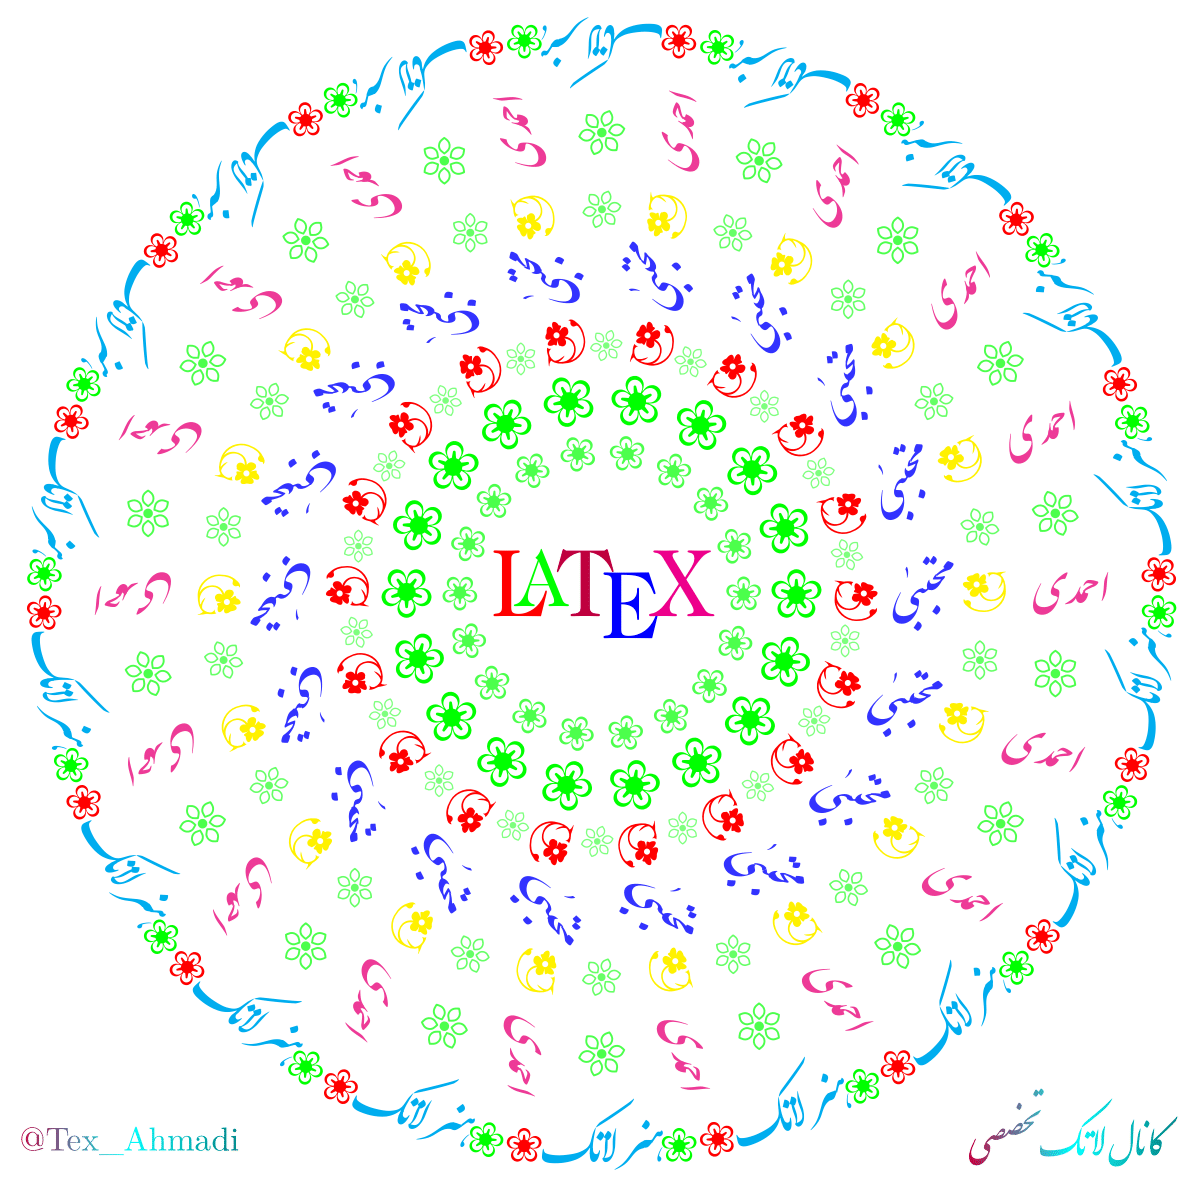
\includegraphics[width=.5cm]{logo1.png}}
%%%%%%%%%%
%حل مشکل در command-Ahmadi
\setbeamertemplate{sections/subsections in toc}[square]
\setbeamertemplate{enumerate items}[square] 

\begin{document}

\begin{frame}
\centerline{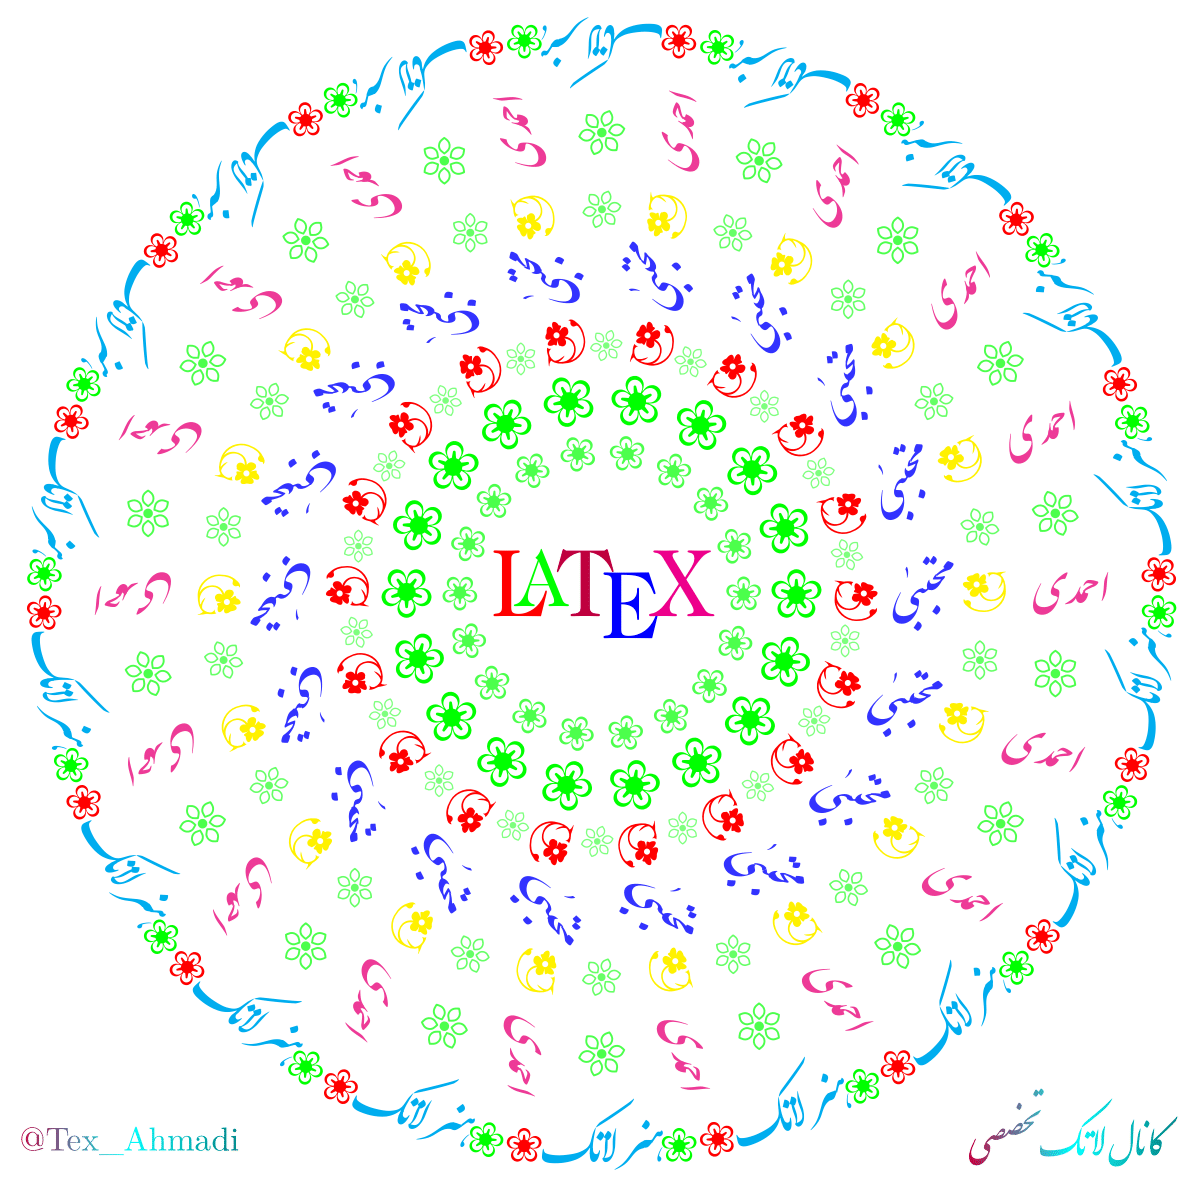
\includegraphics[width=1.5cm]{logo1.png}}
\vskip-1.2\baselineskip
\titlepage
\end{frame}

\begin{frame}
\tableofcontents
\end{frame}

\section{عنوان بخش}
\subsection{زیربخش}
\subsubsection{زیرزیربخش}
\begin{frame}
 توجه: محیط
\lr{enumerate}
\begin{enumerate}\raggedleft
\item 
تست
\item 
متن
\begin{enumerate}\raggedleft
\item 
تست
\item 
متن
\begin{enumerate}\raggedleft
\item 
تست
\end{enumerate}
\end{enumerate}
\end{enumerate}

\end{frame}

\end{document}